\documentclass[11pt]{ltjsarticle}
\usepackage{amsmath}
\usepackage{amssymb}
\usepackage{amsfonts}
\usepackage{physics}
\usepackage{graphicx}
\usepackage{float}
\usepackage{booktabs}
\usepackage{tikz}
\usepackage{xcolor}
\usepackage{pgfplots}
\usepackage{mathcomp}
\usepackage{enumitem}
\usepackage{wrapfig}
\usepackage{etoolbox}
\usepackage{cleveref}
\usepackage[version=4]{mhchem}
\crefformat{figure}{図~#2#1#3}
\crefformat{equation}{式~(#2#1#3)}
\crefformat{table}{表~#2#1#3}
\usetikzlibrary{intersections,calc}
\pgfplotsset{compat=1.18}
\begin{document}
\begin{figure}[H]
  \centering
  \includegraphics[width=0.98\columnwidth]{hyoushi.pdf}
\end{figure}
  \section*{目的}
    各自で作成した単スリット, 複スリットを用いて, 1次元の回折強度分布を測定し, スリットの幅, 間隔を推定する. \\
    実験を通して回折, 干渉現象についての理解を深める. \\
  \section*{原理}
    \begin{figure}[H]
      \centering
      \includegraphics[width=0.5\columnwidth]{LD_fig1.png}
      \caption{スリットによる光回折}
      \label{fig:slit}
    \end{figure}
    \cref{fig:slit}のように波数$k_0$の波がスリットがある壁を通過して距離$L$離れたスクリーンに投影されることを考える. 
    スリット面の点Pでの位置を$X_P$, スクリーン面の点Qでの位置を$X_Q$とおいて, 点Pから点Qまでの距離を$D$とすると, スクリーン上に投影される回折光の振幅$F(X_Q)$はスリット内の各点からの球面上の二次波である素元波の和によって得ることができる.
    ここで各点での入射光の振幅を$A(X_P)$とすると
    \begin{equation}
      F(X_Q) = \int_{\text{スリット部}}A(X_P) \frac{\exp(ik_0 D)}{D} dX_P
      \label{eq:LD1}
    \end{equation}
    と表せる. ここで入射光がスリット分程度の範囲で均一($A(X_P) = A$)であると仮定すると, \cref{eq:LD1}は以下のようになる. 
    \begin{equation}
      F(X_Q) = A\int_{\text{スリット部}} \frac{\exp(ik_0 D)}{D} dX_P
      \label{eq:LD2}
    \end{equation} 
    スリット面とスクリーン間の距離$L$が十分に大きいと仮定するして, \cref{eq:LD2}を近似する.\\
    まず分母について, $D\simeq L$とすると
    \begin{align*}
      F(X_Q) &= A\int_{\text{スリット部}} \frac{\exp(ik_0 D)}{D} dX_P\\
             &\simeq \frac{A}{L} \int_{\text{スリット部}} \exp(ik_0 D) dX_P\\
    \end{align*}
    となる. 次にexpの中身である位相項について, $k_0$との積が大きくなり, $D\simeq L$では十分ではない. そこで以下のように距離$D$を展開し近似することを考える.
    \begin{align*}
      D&=\sqrt{L^2 + (X_Q - X_P)^2}\\
      &=L\qty{1+\frac{1}{2}\frac{(X_Q - X_P)^2}{L^2}-\frac{1}{8}\qty(\frac{(X_Q - X_P)^2}{L^2})^2+\cdots}\\
      &\simeq L\qty{1+\frac{1}{2}\frac{(X_Q - X_P)^2}{L^2}}\\
      &=L\qty(1+\frac{1}{2}\frac{(X_P)^2}{L^2}+\frac{1}{2}\frac{(X_Q)^2}{L^2}-\frac{X_P X_Q}{L^2})\\
      &\simeq L+\frac{{X_Q}^2}{2L}-\frac{X_P X_Q}{L}\\
    \end{align*}
    上式において一回目の近似で$(X_Q - X_P)/L$を十分小さいものとして無視し, 二回目の近似ではスリットの大きさが$L$に比べ十分小さいものとして$({X_P}/L)^2$を無視した.\\
    これらを\cref{eq:LD2}に代入すると
    \begin{align}
      F(X_Q) &=\frac{A}{L}\int_{\text{スリット部}} \exp(i k_0 D) dX_P\notag\\
             &\simeq\frac{A}{L}\int_{\text{スリット部}} \exp\qty(i k_0 \qty(L-\frac{X_P X_Q}{L}+\frac{X_Q^2}{2L}) ) dX_P\notag\\
             &=\frac{A}{L}\int_{\text{スリット部}} \exp\qty(ik_0 \qty(L+\frac{X_Q^2}{2L})) \exp\qty(-i\frac{k_0 X_Q}{L}X_P)dX_P\notag\\
             &=\frac{A}{L}\exp\qty(ik_0 \qty(L+\frac{X_Q^2}{2L}))\int_{\text{スリット部}} \exp\qty(-i\frac{k_0 X_Q}{L}X_P)dX_P\notag\\
      F(X_Q) &\propto \int_{\text{スリット部}} \exp\qty(-i\frac{k_0 X_Q}{L}X_P)dX_P
      \label{eq:LD3}
    \end{align}
    となる. \\

    実際の測定においては回折強度の分布は, 回折光の振幅$F(X_Q)$の二乗で求められる. 幅$w$の単スリットの場合, 
    \begin{align}
      F(X_Q)&\propto\int_{\text{スリット部}} \exp\qty(-i\frac{k_0 X_Q}{L}X_P)dX_P\notag\\
            &=\int_{-w/2}^{w/2}\exp\qty(-i\frac{k_0 X_Q}{L}X_P)dX_P\notag\\
      \therefore|F(X_Q)|^2&\propto\qty(\frac{\sin\qty(\frac{k_0 w}{2L}X_Q)}{\qty(\frac{k_0 w}{2L}X_Q)})^2
      \label{eq:LD4}
    \end{align}
    となる. 同様にスリット間隔$d$でスリット間隔がともに$w$の複スリットの場合, 
    \begin{equation}
      |F(X_Q)|^2\propto\qty(\frac{\sin\qty(\frac{k_0 w}{2L}X_Q)}{\qty(\frac{k_0 w}{2L}X_Q)})^2\cos^2\qty(\frac{k_0 d}{2L}X_Q)
      \label{eq:LD5}
    \end{equation}
    これらの回折強度分布を以下の\cref{fig:graph1}に示す. 
    \begin{figure}[H]
      \centering
      

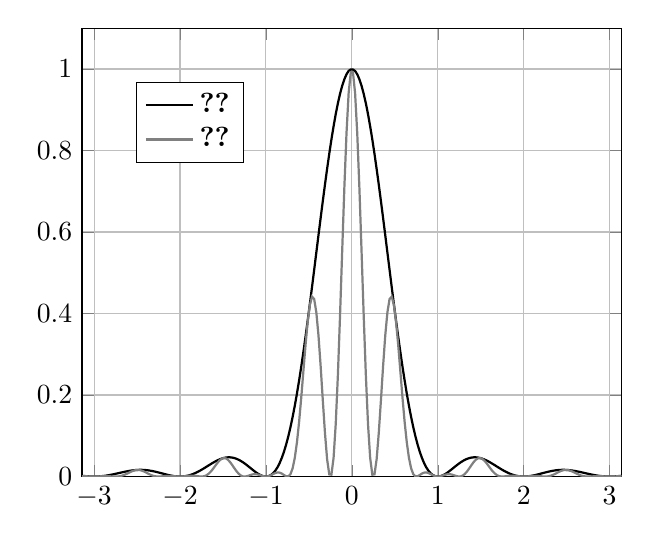
\begin{tikzpicture}
  \begin{axis}[
    samples=400,
    xlabel={},
    ylabel={},
    ymin=0, ymax=1.1,
    xmin=-3.14,xmax=3.14,
    legend style={at={(0.2,0.7)}, anchor=south},
    grid=major,
  ]
    % sinc^2(x)
    \addplot[
      thick
    ] { (sin(deg(pi*x))/(pi*x))^2 };
    \addlegendentry{\cref{eq:LD4}}
    
    % sinc^2(x) * cos^2(x)
    \addplot[
      thick,
      gray
    ] { (sin(deg(pi*x))/(pi*x))^2 * (cos(deg(2*pi*x)))^2 };
    \addlegendentry{\cref{eq:LD5}}
  \end{axis}
\end{tikzpicture}


      \caption{回折強度分布の概形}
      \label{fig:graph1}
    \end{figure}
  \section*{実験}
    \subsection*{実験装置}
      \begin{figure}[H]
        \centering
        \includegraphics[width=0.96\columnwidth]{LD_kigu.png}
        \caption{(a)実験装置の写真, (b)実験装置の概略図}
        \label{fig:kigu}
      \end{figure}
      \noindent \cref{fig:kigu}のような実験装置を用いて, 単スリット, 複スリットの回折強度分布を測定した. \\
      実験装置は, He-Neガスレーザー(波長632.8nm)を光源として, スリットを通過した光をフォトダイオードで受光し, その電流を測定することで回折強度分布を得る.
      \begin{figure}[H]
        \centering
        \begin{minipage}[b]{0.32\columnwidth}
          \centering
          \includegraphics[width=\linewidth]{LD_single.png}
          \caption{単スリットの作成例}
          \label{fig:single}
        \end{minipage}
        \begin{minipage}[b]{0.32\columnwidth}
          \centering
          \includegraphics[width=\linewidth]{LD_double.png}
          \caption{複スリットの作成例}
          \label{fig:double}
        \end{minipage}
      \end{figure}
      \noindent \cref{fig:single},\cref{fig:double}のように, 単スリットはスライドガラスに小さな幅を開けてカッターの刃を固定して作成し, 複スリットは, カッターの間にシャープペンシルの芯をはさんで固定して作成した.
    \subsection*{測定手順}
    \begin{enumerate}
      \item 単スリット, 複スリットをそれぞれ作成した.
      \item スリット間隔をそれぞれ測定した.
      \item \cref{fig:kigu}のような実験装置に単スリットを取付け, 波長632.8nmのHe-Neガスレーザーを照射した.
      \item ステップ幅をそれぞれ0.3mm, 0.1mmとした. 
      \item フォトダイオードを動かしながら信号強度が最も大きくなるところを見つけ, その位置から2ステップ戻して記録を開始した. 
      \item 一次の明線が記録される程度まで記録した. 
      \item スリット, フォトダイオード間の距離を測定した. 
      \item 以上の手順を自作の単スリットと複スリット, 既製品の単スリットと複スリットに対して実施した.
    \end{enumerate}
  \section*{実験結果}
    自作のスリットでの測定結果, フィッティングは以下のようになった.
    \begin{figure}[H]
      \centering
      \begin{minipage}
        [b]{0.48\columnwidth}
        \centering
        \includegraphics[width=\linewidth]{single_jisaku.png}
        \caption{自作単スリットの測定結果}
        \label{fig:single_result}
      \end{minipage}
    \begin{minipage}[b]{0.48\columnwidth}
      \centering
      \includegraphics[width=\linewidth]{double_jisaku.png}
      \caption{自作複スリットの測定結果}
      \label{fig:double_result}
    \end{minipage}
    \end{figure}
    また既製品のスリットでの測定結果, フィッティングは以下のようになった.
    \begin{figure}[H]
      \centering
      \begin{minipage}[b]{0.48\columnwidth}
        \centering
        \includegraphics[width=\linewidth]{single_kisei.png}
        \caption{既製品単スリットの測定結果}
        \label{fig:single_result_seizou}
      \end{minipage}
      \begin{minipage}[b]{0.48\columnwidth}
        \centering
        \includegraphics[width=\linewidth]{double_kisei.png}
        \caption{既製品複スリットの測定結果}
        \label{fig:double_result_seizou}
      \end{minipage}
    \end{figure}
    これらのデータから, スリット幅、スリット間隔は以下のようになった.(スリットとダイオード間の距離の誤差を5cmとした.)
    \begin{table}[H]
      \begin{tabular}{l|c|c}
        スリットの種類 & 幅 $w$ [mm] & スリット間隔 $d$ [mm]\\\hline
        自作単スリット & 0.175\pm 0.008 & -\\\hline
        自作複スリット & 0.111\pm 0.002 & 0.115\pm0.002\\\hline
        既製品単スリット & 0.192\pm 0.009 & -\\\hline
        既製品複スリット & 0.17\pm 0.0018 & 0.28\pm 0.0014\\
      \end{tabular}
    \end{table}
    \section*{課題}
      \subsection*{課題1}
        自作の単スリットの測定した幅$w$は0.203mmであった. また, スリットとダイオード間の距離は1.088mであった.実験後のスリット幅に違いはなかった.\\
        既製品の単スリットの測定した幅$w$は0.2mmであった. また, スリットとダイオード間の距離は1.072mであった.実験後のスリット幅に違いはなかった.
      \subsection*{課題2}
        自作の複スリットの測定した幅$w$は左が0.237mm, 右が0.073mmであった. スリット間距離は0.644mmだった. また, スリットとダイオード間の距離は1.088mであった.実験後のスリット幅に違いはなかった.\\
        既製品の複スリットの測定した幅$w$は左が0.1mm, 右が0.1mmであった.スリット間距離は0.300mmだった. また, スリットとダイオード間の距離は1.072mであった.実験後のスリット幅に違いはなかった.
      \subsection*{課題3}
        1.\cref{eq:LD3}の積分を単スリットについて計算する.
        \begin{align*}
          F(X_Q) &\propto \int_{-w/2}^{w/2} \exp\qty(-i\frac{k_0 X_Q}{L}X_P)dX_P\\
        \end{align*}
        ここで積分公式
        \begin{align*}
          \int_{-a}^{a} e^{-ibx}dx = \int_{-a}^{a} (\cos(bx) - i\sin(bx))dx = 2a\frac{\sin(ba)}{b}(\because \sin(x)\text{は奇関数})
          \label{eq:integral}
        \end{align*}
        を用いると
        \begin{align*}
          F(X_Q) &\propto \int_{-w/2}^{w/2} \exp\qty(-i\frac{k_0 X_Q}{L}X_P)dX_P\\
                 &=\frac{\sin\qty(\frac{k_0 w}{2L}X_Q)}{\qty(\frac{k_0 w}{2L}X_Q)}\\
          \therefore |F(X_Q)|^2 &\propto \qty(\frac{\sin\qty(\frac{k_0 w}{2L}X_Q)}{\qty(\frac{k_0 w}{2L}X_Q)})^2
        \end{align*}
        複スリットについても同様に,スリット中心を$\pm d/2$でとると
        \begin{align*}
          F(X_Q) &\propto \int_{-w/2}^{w/2} \exp\qty(-i\frac{k_0 X_Q}{L}(X_P-\frac{d}{2}))dX_P+\int_{-w/2}^{w/2} \exp\qty(-i\frac{k_0 X_Q}{L}(X_P+\frac{d}{2}))dX_P\\
                 &=\exp\qty(-i\frac{k_0 X_Q}{2L}d+\exp\qty(i\frac{k_0 X_Q}{2L}d))\int_{-w/2}^{w/2} \exp\qty(-i\frac{k_0 X_Q}{L}X_P)dX_P\\
                  &=2\cos\qty(\frac{k_0 d}{2L}X_Q)\int_{-w/2}^{w/2} \exp\qty(-i\frac{k_0 X_Q}{L}X_P)dX_P\\
                  &=2\cos\qty(\frac{k_0 d}{2L}X_Q)\frac{\sin\qty(\frac{k_0 w}{2L}X_Q)}{\qty(\frac{k_0 w}{2L}X_Q)}\\
          \therefore |F(X_Q)|^2 &\propto \qty(\frac{\sin\qty(\frac{k_0 w}{2L}X_Q)}{\qty(\frac{k_0 w}{2L}X_Q)})^2\cos^2\qty(\frac{k_0 d}{2L}X_Q)
        \end{align*}
  \section*{考察}
    今回の実験では, 測定値と実験値の誤差がかなり大きくなってしまった. 計算した誤差から大きく外れた結果になった理由として, 全体的には電圧計の読み方が正確ではなかったことが考えられる. さらに, 自作の複スリットにおいてかなり大きなずれが出たのは, スリット幅が左右で大きく異なっているからだと考えられる. 実際既製品の複スリットではここまで大きなずれがなかったことからも, この要因は大きいと考えられる. 
  \section*{参考文献}
   光回折\_テキスト
   また, コーディングにおいて生成AIを活用した. 
\end{document}